\chapter{Vrednovanje i rezultati} \label{vrednovanja_i_rezultati}

Konačan cilj rada je vrednovati i usporediti algoritme za detekciju društvenih zajednica. U idealnom slučaju postojalo bi proizvoljno mnogo stvarnih primjera društvenih mreža nad kojima bi se algoritmi testirali, no zbog ranije opisanih problema teško je doći do novijih primjera. Time generirane društvene mreže postaju bitne te se koriste kako bi algoritmi bili testirani na što više primjera. Vrednovanje će se provesti nad nekoliko stvarnih primjera mreža i na umjetno stvorenim skupovima podataka. Kroz ovo poglavlje opisat će se korištene evaluacijske mjere, način provođenja testova nad različitim skupovima podataka te dobiveni rezultati kroz.

\section{Evaluacijske mjere}
Za reprezentativnu usporedbu algoritama potrebno je imati više kvalitetnih evaluacijskih mjera koje će pokazati prave odnose meuđu algoritmima nad različitim skupovima podataka. Mjere su osmišljene tako da koriste određena svojstva grafa u  pronađenim konfiguracijama zajednica kao što su stupnjevi vrhova u zajednicama ili bridovi koji se nalaze unutar i među zajednicama. Na temelju njih računaju mjeru koja se koristi za usporedbu. 


\subsection{Modularnost}
Modularnost je mjera kojom se procjenjuje odnos jakosti veza unutar zajednica i jakosti veza među zajednicama. Modularnost se računa prema sljedećoj formuli:
\begin{equation}
	Q = \frac{1}{2m} \sum_{u,v \in V} \bigg[ A_{u,v} - \frac{k_{u}k_{v}}{2m} \bigg] \delta(u,v).
\end{equation}

$m$ predstavlja ukupnu težinu bridova, odnosno broj bridova u bestežinskom grafu. Suma iterira kroz sve parove vrhova, $u$ i $v$. Vrijednost $k_{u}$ je suma svih težina bridova koji izlaze iz grafa, a u ovom slučaju bestežinskog neusmjerenog grafa će biti broj bridova koji su incidentni sa vrhom $u$. Isto vrijedi i za $k_{v}$. $A_{u,v}$ je težina brida između vrhova i iznosi 0 ako vrhovi nisu povezani ili je $u=v$. Funkcija $\delta(u,v)$ govori jesu li promatrani vrhovi u istoj zajednici ili nisu. Iznosi 1 ako jesu, a 0 ako nisu. Vrijednost modularnosti kreće se u intervalu $[ -\frac{1}{2}, 1 ]$. Ako je modularnost 0 ili manje znači da struktura podjele mreže nije jača od slučajne podjele vrhova u zajednice. U slučaju trivijalne podjele mreže u samo jednu zajednicu modularnost će iznositi 0. Što je iznos modularnosti veći to je podjela zajednica u mreži bolja \cite{brandes2007modularity}. Modularnost se koristi u tri od pet algoritama opisanih u radu. Girvan-Newman, Louvain i Leiden algoritam pokušavaju maksimizirati njezinu vrijednost. Vrijednost mjere izračunava se funkcijom definiranom u biblioteci NetworkX pozivom funkcije $nx.algorithms.community.modularity(graph, communities)$



\subsection{Tranzitivnost}
Tranzitivnost se definira kao prosječan koeficijent grupiranja čvorova u grafu. Izračunava se preko formule \ref{eq:triplets}, odnosno kao omjer broja zatvorenih trojki i ukupnog broja trojki u grafu. Tranzitivnost se može promatrati kao vjerojatnost pronalaženja izravne veze između dva vrha ako imaju zajedničkog susjeda. Vrijednost se kreću između 0 i 1. Trojke čvorova u grafovima društvenih mreža su vrlo česti te visoka vrijednost mjere ukazuje da zaista postoje društvene zajednice. No ako je vrijednost mjere niska ne mora nužno vrijediti da ne postoje strukture zajednica. Za izračunavanje mjere koristi se implementacija iz cdlib biblioteke te se prosječna vrijednost tranzitivnosti dobiva pozivom metode $evaluation.avg\_transitivity(graph, communities)$.


\subsection{Veličina zajednice}
Mjera veličina zajednica računa prosječnu veličinu zajednica u grafu. Mjera je vrlo jednostavna i ne otkriva mnogo o kvaliteti podjele zajednica, ali je koristan pokazatelj teži li algoritam pronalaženju većih ili manjih zajednica budući da se za umjetno generirane mreže zna kolike su zajednice veličine. Implementacija iz cdlib biblioteke poziva se naredbom $evaluation.size(graph,communities)$

\pagebreak
\subsection{Omjer vrhova koji sudjeluju u trokutu}
Mjera računa broj čvorova koji se pojavljuju kao dio trokuta u odnosu na ukupan broj čvorova u grafu. Vrijednosti mjere kreću se od 0 do 1 te bi u grafovima društvenih mreža trebale biti što više. Mjera se može iskazati sljedećom formulom:
\begin{equation}
	f(S) = \frac{| \{ u : u \in S, \{(u,v):v, w \in S (u,v) \in E, (u,w) \in E, (v,w) \in E \}  \notin \emptyset \} | }{n_{S}}
\end{equation}
Poziva se iz biblioteke cdlib naredbom \\ $evaluation.triangle\_participation\_ratio(graph, communities).$


\subsection{Prosječna ugrađenost vrhova}
Mjera ugrađenosti procjenjuje u kolikoj mjeri izravni susjedi promatranog vrha pripadaju istoj zajednici. Definirana je kao omjer unutarnjeg stupnja vrha i ukupnog stupnja vrha: 
\begin{equation}
	avg\_embd(c) = \frac{1}{|C|} \sum_{i \in C} \frac{k_{n}^{C}}{k_{n}}.
\end{equation}
Unutarnji stupanj vrha je broj bridova prema vrhovima koji su unutar iste zajednice kao i promatrani vrh. Maksimalna vrijednost ugrađenosti je 1 i postiže se kada su svi susjedi unutar iste zajednice, dok je minimalna vrijednost 0 i događa se u situaciji kada su svi susjedi vrha u nekoj drugoj zajednici. Izračun mjere poziva se naredbom iz biblioteke cdlib: $evaluation.avg\_embeddedness(graph,communities)$.


\subsection{Gustoća bridova unutar zajednica}
Mjerom se izražava koliki dio bridova u grafu povezuje vrhove unutar zajednica u odnosu na ukupan broj mogućih bridova grafa. Vrijednosti se kreću između 0 i 1 te što je mjera bliža 1 konfiguracija podjele zajednica je bolja. Mjera se može izraziti sljedećom formulom:
\begin{equation}
	f(S) = \frac{m_{S}}{\frac{n_{S}(n_{S} - 1)}{2}},
\end{equation}
gdje je $m_{S}$ broj bridova između vrhova unutar zajednica, a donji dio razlomka predstavlja izračun svih mogućih bridova grafa. Mjera se izračunava pozivom metode iz biblioteke cdlib, $evaluation.internal\_edge\_density(g,communities)$


\pagebreak
\subsection{Prosječan unutarnji stupanj}
Prosječan unutarnji stupanj društvene zajednice definira se kao omjer broja bridova unutar zajednice i ukupnog broja vrhova zajednice,
\begin{equation}
	f(S) =  \frac{2m_{s}}{n_{s}}.
\end{equation}
Maksimalna vrijednost mjere iznosi $n_{s} - 1$ u slučaju kada je zajednica potpuno poveza, a minimalna vrijednost će iznositi 0 u slučaju kada nema bridova između čvorova zajednice što upućuje na lošu strukturu zajednice. Mjera se izračunava pozivom metode $evaluation.average\_internal\_degree(g,communities)$ iz cdlib biblioteke.


\subsection{Surprise}
Mjera surprise detaljno je opisana u poglavlju \ref{surprise_alg} o Surprise algoritmu. Mjera je hipergeometrijska distribucija te pretpostavlja da se bridovi između vrhova pojavljuju prema određenoj vjerojatnosti. Osim kao dio algoritma, mjera se može iskoristiti i u evaluaciji gdje što je veći rezultat to je manja vjerojatnost slučajne konfiguracije promatrane zajednice, odnosno da je kvaliteta strukuture zajednice bolja. Izračun mjere obavlja se metodom $evaluation.surprise(graph, communities)$ iz biblioteke cdlib.


\subsection{Provodljivost}
Provodljivost je mjera kojom se iskazuje koliko jako je skup vrhova zajednice povezan s ostatkom mreže. Vrhovi izolirani od grafa imaju nisku vrijednost provodljivosti i čine kvalitetne zajednice. Mjera se može iskazati izrazom:
\begin{equation}
	f(S) = \frac{c_{S}}{2m_{S} + c_{S}},
\end{equation}
gdje je $c_{S}$ broj čvorova zajednice, a $m_{S}$ broj bridova unutar zajednice. Vrijednosti se kreću između 0 i 1 te je struktura zajednica bolja što je vrijednost provodljivost niža. Mjera se izračunava pozivom sljedeće metode iz biblioteke cdlib: $evaluation.conductance(graph, communities)$.


\pagebreak
\section{Vrednovanje algoritama}
Pomoću opisanih mjera usporedit će se karakteristike promatranih algoritama te će se pokušati zaključiti u kojim situacijama je određeni algoritam bolji ili lošiji. Postupak vrednovanja algoritama odvijat će kroz tri testa.  Prva dva testa odvijaju se na umjetno generiranim skupovima podatka, a treći test je proveden nad stvarnim podacima.

\subsection{Umjetni skupovi podataka}
U prvom testu svih 5 algoritama pokrenut će se nad skupovima podataka od 100, 200, 300, 400 i 500 čvorova. Primjeri mreža su umjetno generirani Watts-Strogatz modelom, gdje svaki čvor u prosjeku ima 20 susjeda te je vjerojatnost prespajanja brida 0.1. Za svaku veličinu mreže generirano je 5 primjera te su rezultati uprosječeni. Na slici \ref{fig:test1} vidljivi su rezultati izvršavanja algoritama i izračuna evaluacijskih mjera. Može se primijetiti kako je Girvan-Newannov algoritam lošiji od ostalih algoritama prema gotovo svim mjerama. Postoje iznimke u modularnosti i surprise mjeri, ali u mjeri omjera vrhova u trokutovima i  mjeri provodljivosti pokazuje značajno slabije rezultate od ostalih. Osim prema evaluacijskim mjerama, Girvan-Newman algoritam je pokazao i veliku vremensku složenost te kako se povećava broj vrhova u mreži tako se značajno produžuje vremensko izvođenje u usporedbi s ostalim algoritmima. Time se može zaključiti kako bi provođenje Girvan-Newmanovog algoritma bilo previše vremenski zahtjevno za pokretanje nad grafovima od nekoliko tisuća čvorova te ga se neće pokretati na većim primjerima grafova. Najbolje rezultate u većini mjera pokazao je Louvain algoritam. U mjeri veličine zajednica najbolje rezultate pokazao je Surprise algoritam, dok ostali algoritmi imaju tendenciju precjenjivanja ili podcjenjivanja veličine.

\begin{figure}
	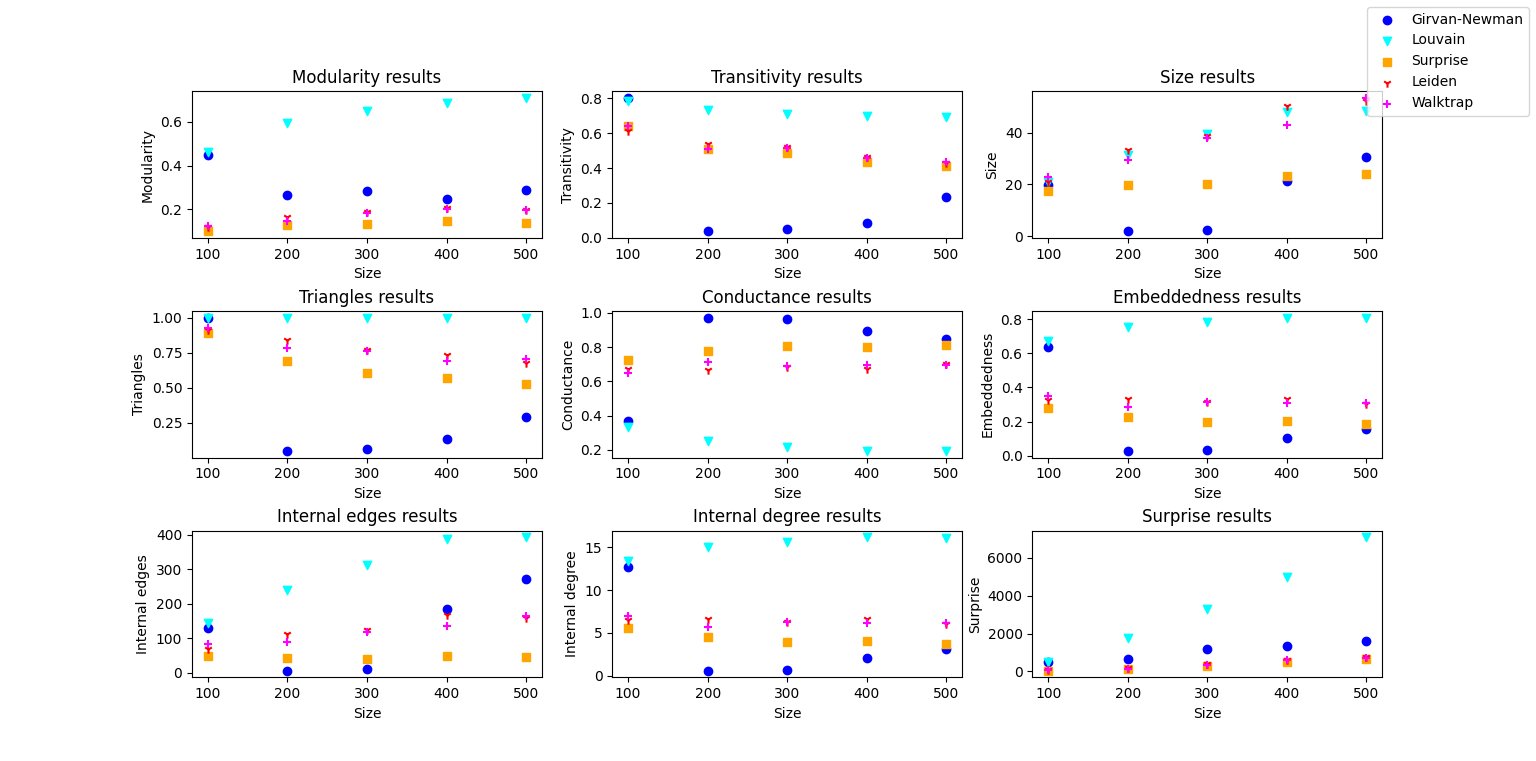
\includegraphics[width=\linewidth]{images/test1.png}
	\caption{Rezultati evaluacije algoritama nad skupovima od 100, 200, 300, 400 i 500 čvorova. Čvorovi imaju u prosjeku 20 susjeda. Na x-osi su veličine grafova, a na y-osi skale pojedinih evaluacijskih mjera.}
	\label{fig:test1}
\end{figure}


%\pagebreak
Zbog navedenih razloga u vezi nedostataka Girvan-Newman algoritma drugi i treći test odvijat će se samo na ostalim algoritmima. Drugi test je podijeljen na dva dijela te se vrednovanje provodi na grafovima od 1000, 5000, 10 000, 20 000 i 40 000 čvorova. U prvom dijelu grafovi se sastoje od vrhova koji u prosjeku imaju 10 susjeda, a u drugom dijelu grafovi imaju 100 susjeda u prosjeku.  Vjerojatnost prespajanja bridova je 0.1. Cilj je usporediti ponašanje algoritama na većim skupovima podataka i različitim veličinama zajednica. Na slikama \ref{fig:test2_10} i \ref{fig:test2_100} vidljivi su rezultati evaluacijskih mjera nakon izvođenja algoritama. Može se primijetiti kako se na oba testa dolazi do sličnih rezultata. Na većini mjera Louvain algoritam daje značajno bolje rezultate te kvaliteta evaluacijskih mjera raste s porastom veličine mreže. Može se primijetiti kako Louvain i Leiden u oba slučaja precjenjuju veličine zajednica. Walktrap algoritam ih je precjenjivao za skupove podataka od 100 susjeda, a u skupovima od 10 susjeda daje dobre procjene. Surprise algoritam pokazuje najbolje rezultate u oba slučaja. Što se tiče većeg skupa podataka, može se primijetiti kako na mjerama tranzitivnosti, omjera vrhova u trokutima i mjeri prosječnog unutarnjeg stupnja za sve algoritme, osim Louvain, rezultati evaluacijskih mjera pokazuju značajan pad tijekom porasta veličine mreže. Za mjeru gustoće bridova unutar zajednica može se zaključiti kako je u korelaciji sa mjerom veličine zajednica jer je tada više bridova u zajednici, ali rezultati pokazuju da iako Leiden algoritam pronalazi veće zajednice, njihova podjela ipak nije toliko kvalitetna kao u slučaju Louvain algoritma. Mjera surprise pokazuje da iako je tijekom postupka pronalaženja zajednica Surprise algoritam maksimizira ipak ne daje bolje rezultate od ostalih algoritama, gdje Louvain algoritam ponovno daje puno značajno rezultate od ostalih algoritama. Prema rezultatima evaluacijskih mjera najlošije rezultate ostvaruje Surprise algoritam, dok je Leiden algoritam na većini mjera ipak nešto bolji od Walktrapa. Na većim mrežama i sa većim brojem susjeda složenost Walktrap algoritma dolazi do izražaja kada njegovo izvođenje postaje značajno duže od izvođenja ostalih algoritama.

\begin{figure}
	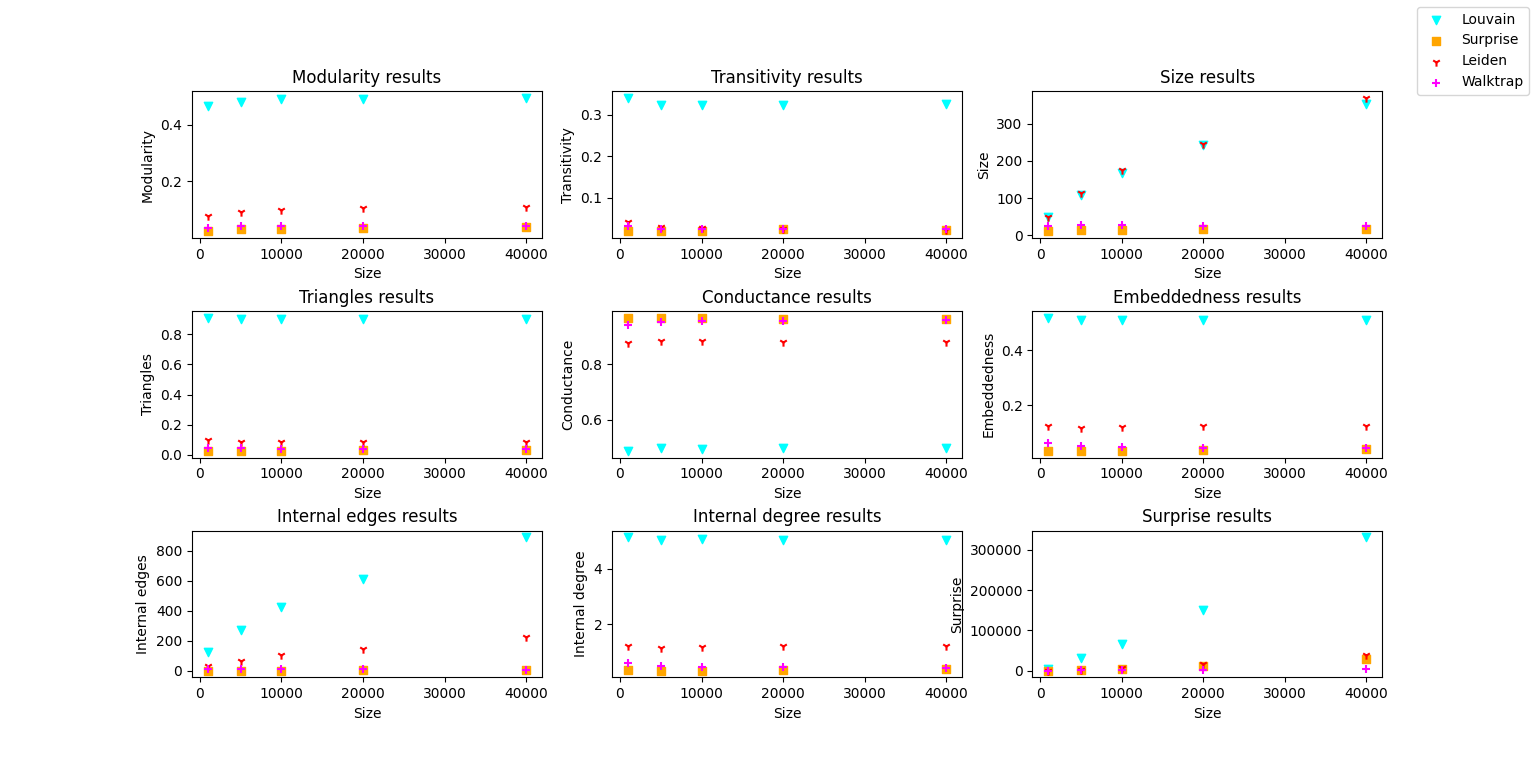
\includegraphics[width=\linewidth]{images/test2_10.png}
	\caption{Rezultati evaluacije algoritama nad skupovima od 1000, 5000, 10 000, 20 000 i 40 000 čvorova. Čvorovi imaju u prosjeku 10 susjeda. Na x-osi su veličine grafova, a na y-osi skale pojedinih evaluacijskih mjera.}
	\label{fig:test2_10}
\end{figure}

\begin{figure}
	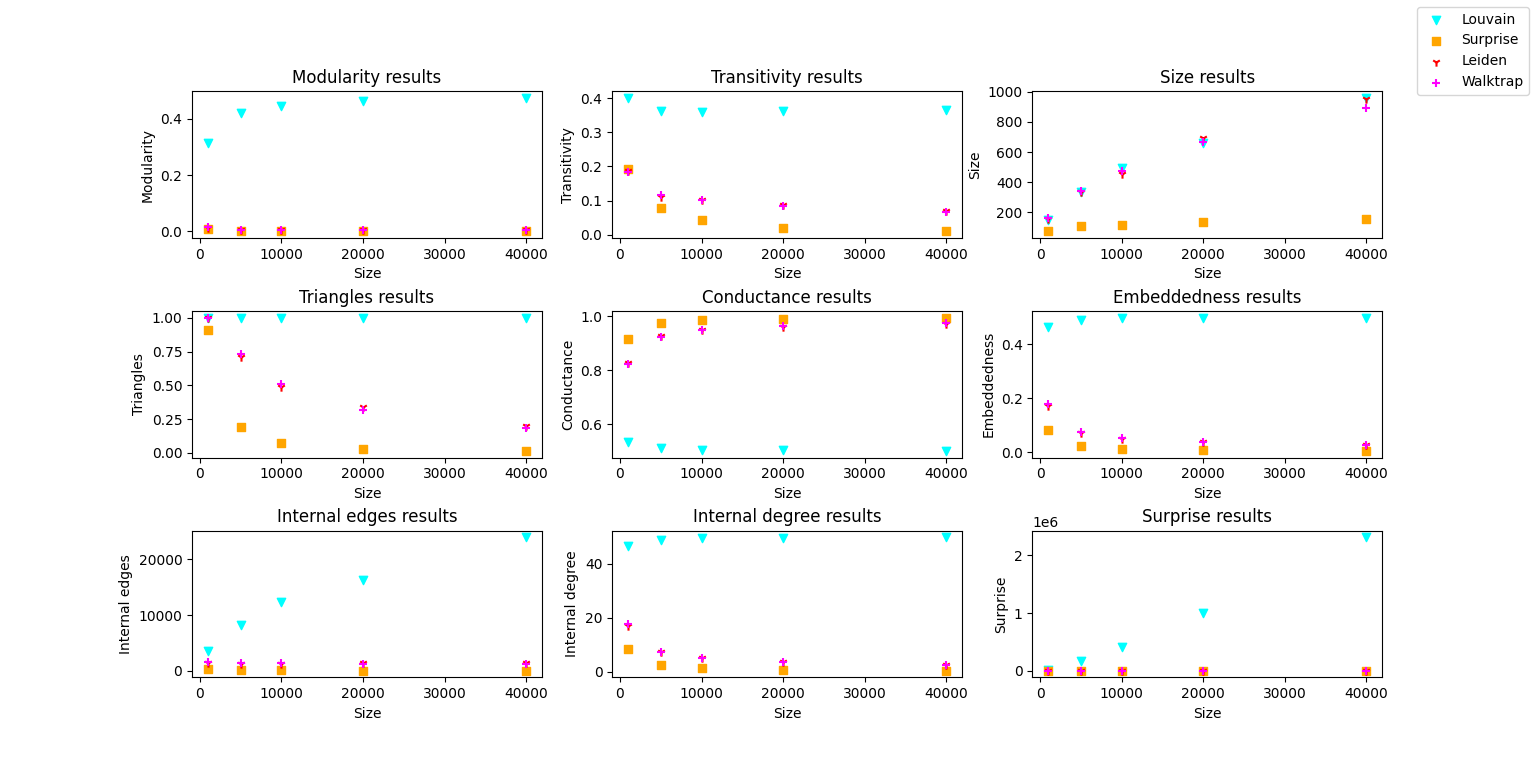
\includegraphics[width=\linewidth]{images/test2_100.png}
	\caption{Rezultati evaluacije algoritama nad skupovima od 1000, 5000, 10 000, 20 000 i 40 000 čvorova. Čvorovi imaju u prosjeku 100 susjeda. Na x-osi su veličine grafova, a na y-osi skale pojedinih evaluacijskih mjera.}
	\label{fig:test2_100}
\end{figure}


\section{Stvarni skupovi podataka}

Posljednji test vrednovanja algoritama provodi se pomoću stvarnih skupova podataka. Na 5 primjera društvenih mreža, opisanih u poglavlju \ref{real_data}, usporedit će se rezultati evaluacijskih mjera. Mreže su različitih veličina, od najmanje sa 4039 vrhova do najveće sa 143 884 vrhova.

Na slici \ref{fig:test3} vidljivi su rezultati evaluacijskih mjera za pronađene konfiguracije zajednica. Iako su skupovi podataka različitih dimenzija i karakteristika mogu se primijetiti uzorci u ponašanju algoritama. Louvain algoritam daje značajno bolje rezultate od ostalih algoritama na svim evaluacijskim mjerama za koje se zna kakvi koeficijenti znače bolji rezultat. Louvain i Leiden ponovno daju veće vrijednosti u procjeni veličine zajednica što znači da ih, prema zaključcima sa prošlih skupova podataka, precjenjuju u veličini. Među preostalim algoritama Leiden se ističe od Walktrap i Surprise algoritama na određenim skupovima podataka i mjerama, a najviše na skupu facebook1. Mjere nad stvarnim skupovima podataka ponovno pokazuju kako se razlika među rezultatima evaluacijskih mjera značajno povećava s porastom veličine zajednica. Primijećen je i utjecaj složenosti Walktrap algoritma koji se otkriva u većim mrežama gdje izvođenje algoritma traje značajno dulje.


\begin{figure}
	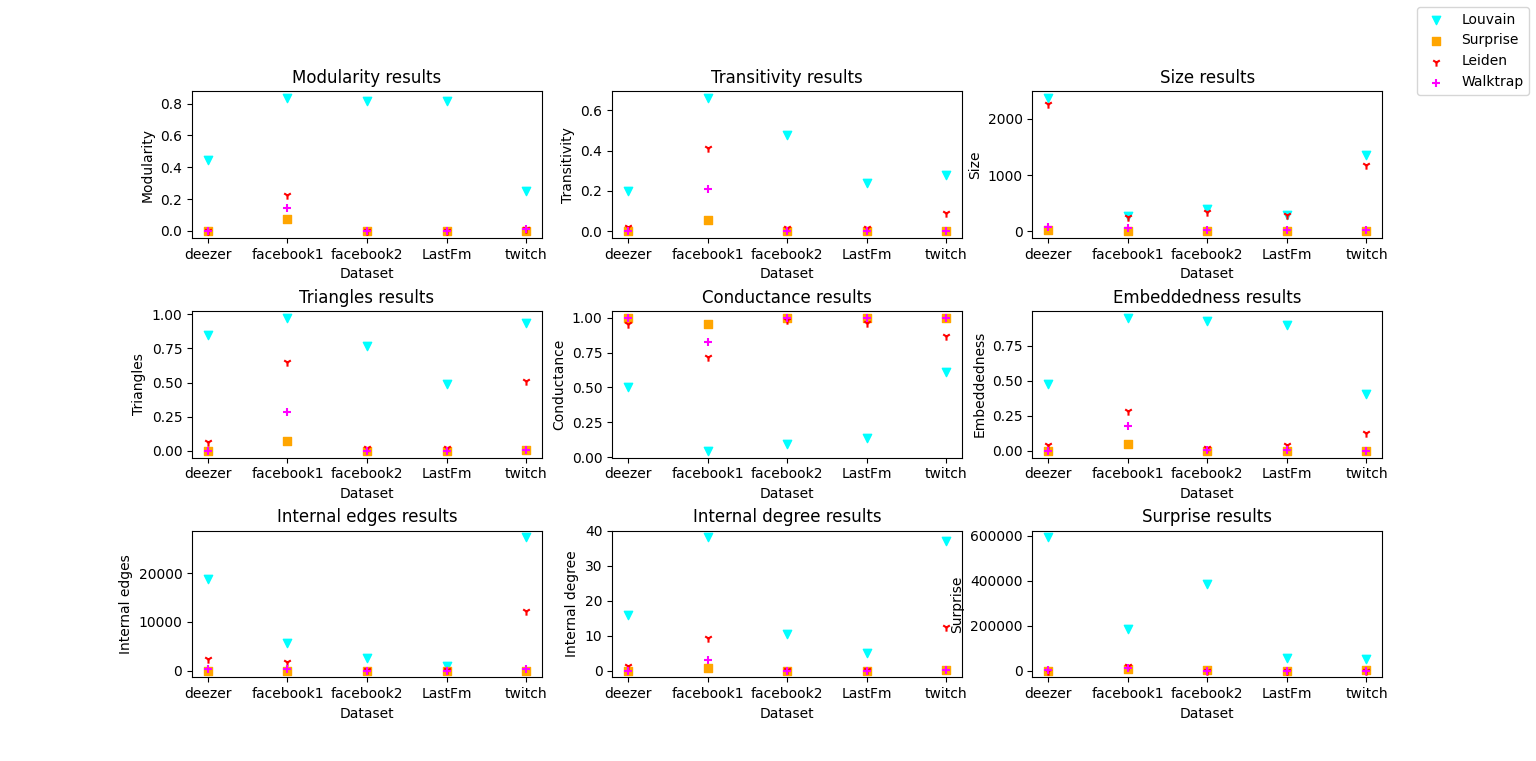
\includegraphics[width=\linewidth]{images/test3.png}
	\caption{Rezultati evaluacije algoritama nad stvarnim skupovima. Podaci su sa društvenih mreža: Deezer, dva skupa podataka sa Facebooka, LastFM i Twitch. Na x-osi su imena društvenih mreža, a na y-osi skale pojedinih evaluacijskih mjera.}
	\label{fig:test3}
\end{figure}


Na slici \ref{fig:facebook_res} mogu se detaljnije promotriti brojčane vrijednosti za izvršavanje algoritama nad facebook1 skupom podataka. Postoji značajna razlika koja dijeli Leiden algoritam od preostalih algoritama. Problem Surprise i Walkrap algoritma najviše se očituje u pronalasku vrlo malih zajednica koje ne mogu biti evaluirane s visokim rezultatima. Louvain algoritam precjenjuje veličine zajednica, ali tada se više zajednica prikladne veličine može naći u istoj zajednici što na kraju neće imati toliko utjecaja i ostvarit će bolje rezultate u evaluaciji ostalih mjera.



\begin{figure}
	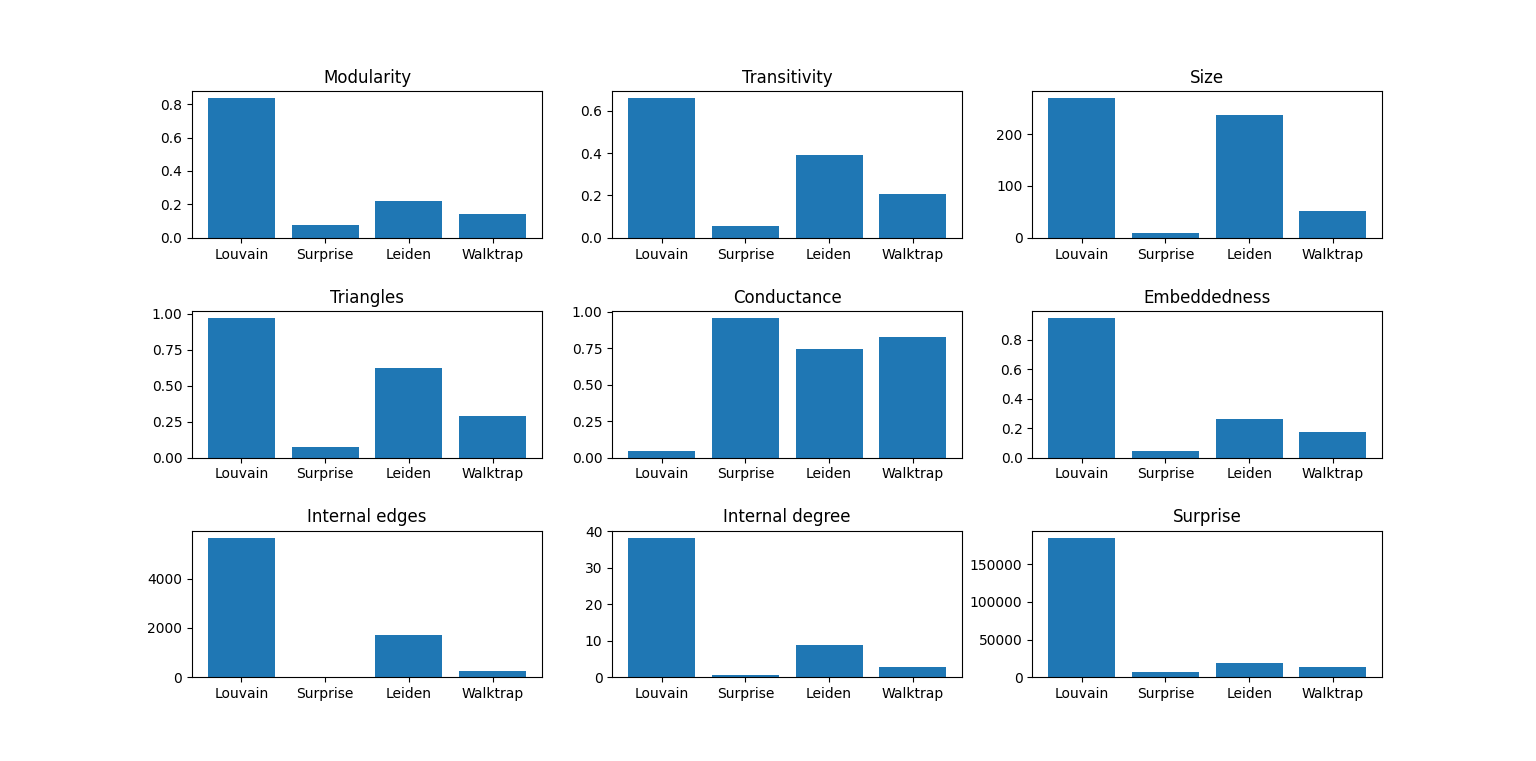
\includegraphics[width=\linewidth]{images/facebook1.png}
	\caption{Usporedba rezultata evaluacije algoritama nad društvenom mrežom Facebook od 4039 vrhova. Na x-osi su imena algoritama, a na y-osi skale pojedinih evaluacijskih mjera.}
	\label{fig:facebook_res}
\end{figure}